\begingroup\hyphenpenalty=10000\relax
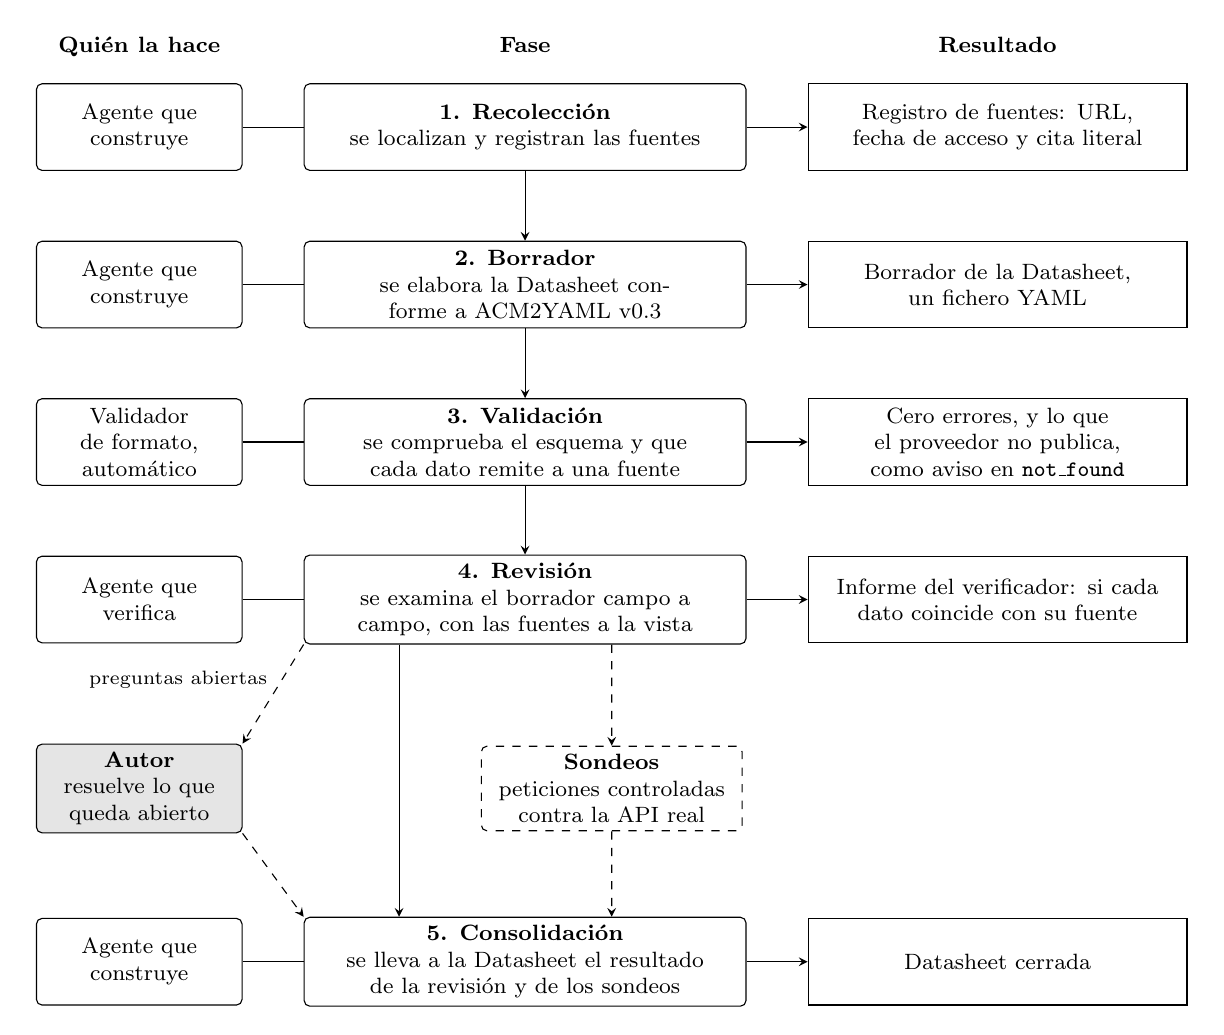
\begin{tikzpicture}[
  font=\footnotesize,
  quien/.style={draw, rounded corners=2pt, align=center, text width=24mm, minimum height=11mm, inner sep=3pt},
  fase/.style={draw, rounded corners=2pt, align=center, text width=54mm, minimum height=11mm, inner sep=3pt},
  sale/.style={draw, align=center, text width=46mm, minimum height=11mm, inner sep=3pt},
  desvio/.style={draw, dashed, rounded corners=2pt, align=center, text width=31mm, inner sep=3pt},
  cabecera/.style={font=\footnotesize\bfseries, align=center, anchor=base}
]
\node[cabecera, text width=26mm] at (1.4,0.95) {Quién la hace};
\node[cabecera, text width=56mm] at (6.3,0.95) {Fase};
\node[cabecera, text width=48mm] at (12.3,0.95) {Resultado};
\node[quien] (q1) at (1.4,0) {Agente que construye};
\node[quien] (q2) at (1.4,-2.0) {Agente que construye};
\node[quien] (q3) at (1.4,-4.0) {Validador de formato, automático};
\node[quien] (q4) at (1.4,-6.0) {Agente que verifica};
\node[quien, fill=gray!20] (autor) at (1.4,-8.4) {\textbf{Autor}\\ resuelve lo que queda abierto};
\node[quien] (q5) at (1.4,-10.6) {Agente que construye};
\node[fase] (f1) at (6.3,0) {\textbf{1. Recolección}\\ se localizan y registran las fuentes};
\node[fase] (f2) at (6.3,-2.0) {\textbf{2. Borrador}\\ se elabora la Datasheet conforme a ACM2YAML v0.3};
\node[fase] (f3) at (6.3,-4.0) {\textbf{3. Validación}\\ se comprueba el esquema y que cada dato remite a una fuente};
\node[fase] (f4) at (6.3,-6.0) {\textbf{4. Revisión}\\ se examina el borrador campo a campo, con las fuentes a la vista};
\node[fase] (f5) at (6.3,-10.6) {\textbf{5. Consolidación}\\ se lleva a la Datasheet el resultado de la revisión y de los sondeos};
\node[desvio] (sondeo) at (7.4,-8.4) {\textbf{Sondeos}\\ peticiones controladas contra la API real};
\node[sale] (r1) at (12.3,0) {Registro de fuentes: URL, fecha de acceso y cita literal};
\node[sale] (r2) at (12.3,-2.0) {Borrador de la Datasheet, un fichero YAML};
\node[sale] (r3) at (12.3,-4.0) {Cero errores, y lo que el proveedor no publica, como aviso en \texttt{not\_found}};
\node[sale] (r4) at (12.3,-6.0) {Informe del verificador: si cada dato coincide con su fuente};
\node[sale] (r5) at (12.3,-10.6) {Datasheet cerrada};
\foreach \i in {1,...,5} { \draw (q\i.east) -- (f\i.west); }
\foreach \i in {1,...,5} { \draw[-stealth] (f\i.east) -- (r\i.west); }
\draw[-stealth] (f1.south) -- (f2.north);
\draw[-stealth] (f2.south) -- (f3.north);
\draw[-stealth] (f3.south) -- (f4.north);
\draw[-stealth] ([xshift=-16mm]f4.south) -- ([xshift=-16mm]f5.north);
\draw[-stealth, dashed] ([xshift=11mm]f4.south) -- (sondeo.north);
\draw[-stealth, dashed] (sondeo.south) -- ([xshift=11mm]f5.north);
\draw[-stealth, dashed] (f4.south west) -- node[midway, above left, font=\scriptsize, inner sep=2pt] {preguntas abiertas} (autor.north east);
\draw[-stealth, dashed] (autor.south east) -- (f5.north west);
\end{tikzpicture}
\endgroup
